% Based on CS224R: Default Project LaTeX template https://drive.google.com/file/d/1TdXav51fMSQPjT83Ajdz3ZRRMB6xnhjB/view?usp=sharing?
% !TeX root = final-report.tex

\documentclass{article}

\usepackage[preprint]{cs224r_2025}
\usepackage[utf8]{inputenc}
\usepackage[T1]{fontenc}
\usepackage{hyperref}
\usepackage{url}
\usepackage{booktabs}
\usepackage{amsfonts}
\usepackage{nicefrac}
\usepackage{microtype}
\usepackage{xcolor}
\usepackage{amsmath}
\usepackage{graphicx}
\usepackage{lipsum}
\usepackage{algorithm}
\usepackage{algpseudocode}
\usepackage{listings}
\usepackage{color}
\usepackage{graphicx}
\usepackage{caption}

\definecolor{codebg}{RGB}{245,245,244}
\lstdefinestyle{python}{
  backgroundcolor=\color{codebg},
  language=Python,
  basicstyle=\ttfamily\footnotesize,
  keywordstyle=\color{blue!80!black},
  commentstyle=\color{green!50!black},
  stringstyle=\color{red!70!black},
  showstringspaces=false,
  columns=fullflexible,
  keepspaces=true,
  frame=single,
  breaklines=true,
  breakatwhitespace=true,
  tabsize=4,
  captionpos=b
}


\begin{document}

% ============================================================================
% PART 1: ONE-PAGE EXTENDED ABSTRACT
% ============================================================================
\begin{titlepage}
\begin{center}
\Large\textbf{Extended Abstract}
\end{center}
\vspace{10pt}

\paragraph{Motivation} Despite their general capabilities, Large Language Models (LLMs) struggle with multi-step numerical reasoning tasks. The Countdown puzzle exemplifies this challenge, requiring models to combine integers using arithmetic operations to exactly reach a target integer. Even state of the art small instruction-tuned models like \texttt{Qwen2.5-0.5B-Instruct} achieve 0\% accuracy on our Countdown benchmark, necessitating specialized fine-tuning to develop these reasoning capabilities. While REINFORCE Leave-One-Out (RLOO) offers an efficient alternative to PPO for such specialized fine-tuning, it suffers from sparse rewards when models rarely generate correct solutions. This creates a vicious cycle: RLOO cannot estimate meaningful advantage baselines without correct samples, preventing the model from improving. We propose Adaptive-Temperature Ladder Sampling (ATLaS) to break this cycle by more systematically exploring the solution space.

\paragraph{Method} ATLaS extends RLOO by introducing an adaptive temperature control mechanism that activates when initial sampling fails to produce a correct solution. The algorithm operates in a ladder fashion: starting with a base temperature $\tau_0$, it incrementally increases temperature by $\Delta\tau$ up to $M$ attempts while the number of correct samples for a given prompt is below a threshold $C_{min}$. Unlike fixed high-temperature sampling, ATLaS maintains low temperatures when the model performs well, preserving sample quality while pursuing signal for more difficult problems. The integration with RLOO's multi-sample advantage requires only modification of the sampling phase while preserving the core variance reduction benefits.

\paragraph{Implementation} We implement ATLaS within a custom RLOO training framework. Our implementation efficiently resamples only prompts lacking a correct solution, minimizing computational overhead. Key hyperparameters tested in our experiments: base temperature $\tau_0=0.7$, increment $\Delta\tau=0.1$, maximum attempts $M=3$, and minimum correct samples $C_{min}=1$. 

\paragraph{Results} On our Countdown benchmark, the RLOO model trained with ATLaS achieves 0.683 score compared to 0.647 for vanilla RLOO, representing an 8.4\% relative improvement in a single-run evaluation. Analysis reveals that 37.9\% of prompts initially lack correct solutions (noting that our strong SFT baseline already achieves a 0.406 score , so rewards are not truly sparse). ATLaS successfully recovers 11.4\% of these through temperature adaptation. Due to computational constraints limiting us to single runs, these results should be considered preliminary findings requiring validation through repeated experiments to establish statistical significance.

\paragraph{Discussion} ATLaS demonstrates that simple algorithmic modifications can help address challenges in RL-based LLM fine-tuning. While our evaluation focuses on Countdown tasks, the approach generalizes to any online sparse-reward scenario where increased sampling diversity can reveal solution paths. Future work could explore dynamic sample size adjustment and application to broader mathematical reasoning benchmarks.

\paragraph{Conclusion} We introduce ATLaS, an adaptive temperature control mechanism that enhances RLOO's effectiveness on sparse-reward tasks. By systematically increasing exploration when needed, ATLaS recovers training signals from previously intractable problems, achieving an 8.4\% relative improvement on our Countdown benchmark. This work demonstrates that addressing the exploration-exploitation trade-off through adaptive sampling can improve RL fine-tuning for challenging reasoning tasks.

\end{titlepage}

% ============================================================================
% PART 2: MAIN PAPER
% ============================================================================

\begin{center}
\rule{\linewidth}{1.5pt}
\vspace{0.8em}

\raisebox{-0.3em}{
\includegraphics[height=1.5em]{ladder.png}}\hspace{0.5em}%
{\Large\bfseries Adaptive Temperature Ladder Sampling (ATLaS) for REINFORCE Leave-One-Out (RLOO) \par}
\vspace{0.6em}

\textit{A \href{https://cs224r.stanford.edu/material/CS224R_Default_Project_Guidelines.pdf}{default project} for CS 224R: Deep Reinforcement Learning}

\vspace{0.8em}
\rule{\linewidth}{1.5pt}
\end{center}

\begin{center}
\textbf{Jonathan Algar} \\[0.5em]
Non-Degree Student, Stanford Center for Global \& Online Education\\[0.3em]
\texttt{\href{mailto:jonathan.algar@stanford.edu}{jalgar@stanford.edu}}
\end{center}


\begin{abstract}
REINFORCE Leave-One-Out (RLOO) offers an efficient alternative to PPO for Large Language Model (LLM) fine-tuning but suffers from sparse rewards in mathematical reasoning tasks where correct solutions are rare. We introduce \textbf{Adaptive-Temperature Ladder Sampling (ATLaS)}, a simple yet effective extension that systematically increases sampling temperature when correct solutions are not found, recovering training signals from previously intractable problems. Our approach uses temperature as an exploration mechanism while maintaining sample quality when the model performs well. On our Countdown benchmark, ATLaS improves the score by a relative 8.4\% over vanilla RLOO by successfully solving 11.4\% of problems that generate zero correct solutions under fixed sampling. This work demonstrates that addressing the exploration-exploitation trade-off through adaptive temperature control can enhance RL-based fine-tuning for challenging reasoning tasks.
\end{abstract}

\section{Introduction}
Large Language Models (LLMs) demonstrate remarkable capabilities across diverse tasks, yet continue to struggle with multi-step numerical reasoning problems. The Countdown puzzle exemplifies this challenge: given a small set of integers (for example, \{4, 31, 35, 62\}), the task requires combining them with basic arithmetic operations to exactly reach a target integer (for example, 41). Despite its apparent simplicity, both base and instruction-tuned versions of small models like \texttt{Qwen2.5-0.5B} achieve zero accuracy our Countdown benchmark without specialized fine-tuning.

Reinforcement learning from human feedback (RLHF) has become an important technique for improving LLM capabilities beyond supervised fine-tuning~\cite{ouyang2022training}. Among RL algorithms for LLM fine-tuning, REINFORCE Leave-One-Out (RLOO)~\cite{ahmadian2024back} offers an attractive balance of simplicity and effectiveness, requiring 50-70\% less memory than Proximal Policy Optimization (PPO) while achieving competitive performance. However, RLOO faces a significant limitation when applied to tasks with sparse rewards: without sufficient correct samples to estimate meaningful advantage baselines, the algorithm cannot differentiate between attempts of varying quality.

In this work, we propose Adaptive-Temperature Ladder Sampling (ATLaS), a simple modification to RLOO that addresses the sparse reward challenge through intelligent exploration. Our key insight is that temperature control in language model sampling can serve as an effective exploration mechanism: while low temperatures preserve high-quality samples when the model performs well, strategically increasing temperature when correct solutions are absent can reveal previously hidden solution paths.

\section{Related work}

\subsection{Supervised Fine-Tuning (SFT)}

Supervised fine-tuning forms the foundation for subsequent RL-based methods. The standard RLHF pipeline begins with SFT on high-quality demonstrations~\cite{ouyang2022training}, which proves particularly important for mathematical reasoning tasks. Recent work by ~\cite{dong2023abilities} shows that mathematical capabilities improve consistently with increasing data quantity, though general abilities plateau after approximately 1000 examples. This highlights the importance of specialized datasets for mathematical tasks.

\subsection{REINFORCE Leave-One-Out (RLOO)}

RLOO represents a significant advancement in policy gradient methods for LLM fine-tuning. Initially proposed by ~\cite{kool2019buy} for combinatorial optimization, RLOO was adapted for LLM fine-tuning by ~\cite{ahmadian2024back}. The key innovation lies in its variance reduction technique: for each sample in a batch, RLOO uses the average reward of all other samples as a baseline.

The theoretical foundation of RLOO builds on the insight that multiple samples from the current policy can serve dual purpose: contributing to gradient estimation while simultaneously providing baselines for variance reduction. Recent implementations have shown that RLOO achieves performance comparable to PPO while using 50-70\% less vRAM and running 2-3x faster~\cite{huang2024putting}.

\subsection{Temperature control in LLMs}

Temperature sampling has long been recognized as important for controlling LLM output diversity~\cite{graves2013generating}. In the softmax function, temperature $\tau$ scales the logits: $p_i = \exp(z_i/\tau) / \sum_j \exp(z_j/\tau)$. Lower temperatures concentrate probability mass on high-likelihood tokens, while higher temperatures increase diversity.

Recent work explores adaptive temperature control for various applications. ~\cite{zhu2024hot} propose learning token-wise temperature controllers for code generation, while \cite{renze2024effect} investigate temperature scheduling for improved sample quality. However, these approaches typically focus on inference-time generation rather than train-time exploration. Our work differs by coupling temperature adaptation with RL's reward signal, using it as an exploration mechanism during policy optimization.

\subsection{Addressing sparse rewards in RL}

The sparse reward problem is well-documented in RL literature. Traditional approaches include reward shaping~\cite{ng1999policy}, curriculum learning~\cite{bengio2009curriculum}, and exploration bonuses~\cite{bellemare2016unifying}. 

For LLMs specifically, ~\cite{lightman2023let} introduce process supervision, providing intermediate rewards during mathematical reasoning. However, this requires expensive step-by-step annotations. Self-rewarding mechanisms ~\cite{chen2024self} offer an alternative but rely on fixed heuristics that may not generalize across problem types.

Our approach requires no additional annotations or reward engineering while maintaining the simplicity of outcome-based rewards.

\section{Method}

\subsection{RLOO foundation}

RLOO operates by generating $K$ samples $\{y_1, ..., y_K\}$ for each prompt $x$ and computing advantages using leave-one-out baselines:

\begin{equation}
b(x, y_k) = \frac{1}{K-1}\sum_{i=1, i \neq k}^{K} R(x, y_i)
\end{equation}

The policy gradient update follows:
\begin{equation}
\label{eq:grad}
\nabla_\theta J(\theta) = \mathbb{E}_{x \sim \mathcal{D}} \left[\frac{1}{K}\sum_{k=1}^{K} A(x, y_k) \nabla_\theta \log \pi_\theta(y_k|x)\right]
\end{equation}

This formulation provides unbiased gradient estimates while leveraging all samples for variance reduction.

\subsection{The ATLaS algorithm}

ATLaS extends RLOO by introducing adaptive temperature control during sampling. The key insight is that when initial sampling at base temperature $\tau_0$ fails to produce correct solutions, incrementally increasing temperature can reveal solution paths while maintaining overall sample quality.

\begin{algorithm}[H]
\caption{Adaptive-Temperature Ladder Sampling (ATLaS)}
\label{alg:atlas}
\begin{algorithmic}[1]
\Require Prompts $\{x_1, \ldots, x_B\}$; base temperature $\tau_0$; increment $\Delta\tau$; max attempts $M$; min correct samples $C_{min}$
\Ensure Samples and advantages for each prompt
\For{each prompt $x_i$}
    \State $\mathcal{S}_i \gets \emptyset$ \Comment{Initialize sample set}
    \For{$m = 0$ to $M-1$}
        \State $\tau_m \gets \tau_0 + m \cdot \Delta\tau$
        \State Generate $K$ samples $\{y_1^{(m)}, ..., y_K^{(m)}\} \sim \pi_\theta(\cdot|x_i, \tau_m)$
        \State Compute rewards $\{r_1^{(m)}, ..., r_K^{(m)}\}$
        \State $C_i^{(m)} \gets |\{j : r_j^{(m)} = 1.0\}|$ \Comment{Count correct samples}
        \If{$C_i^{(m)} \geq C_{min}$ \textbf{or} $m = M-1$}
            \State $\mathcal{S}_i \gets \{y_1^{(m)}, ..., y_K^{(m)}\}$
            \State \textbf{break}
        \EndIf
    \EndFor
    \State Compute RLOO advantages for $\mathcal{S}_i$ per Eq~\ref{eq:grad}
\EndFor
\end{algorithmic}
\end{algorithm}

\subsubsection{Design choices}

Several design choices in ATLaS merit explanation:

\textbf{Linear temperature schedule}: We use a simple linear increase ($\tau_m = \tau_0 + m\Delta\tau$) rather than exponential or learned schedules. This provides predictable exploration increases while maintaining interpretability.

\textbf{Prompt level adaptation}: Temperature adaptation occurs per prompt rather than per batch or globally. This allows the algorithm to adapt to varying problem difficulties within a single batch.

\textbf{Early stopping}: Once sufficient correct samples are found, we stop increasing temperature. This preserves sample quality for problems the model can already solve.

\textbf{Fixed sample size}: We maintain $K$ samples regardless of temperature, ensuring consistent advantage estimation across all prompts.

\subsubsection{ATLaS Integration with RLOO}

Our implementation modifies the standard RLOO training loop to incorporate ATLaS while maintaining computational efficiency. The key optimization is selective resampling:

\begin{lstlisting}[style=python]
for idx, (samples, rewards) in enumerate(zip(all_samples, all_rewards)):
    correct_count = sum(1 for r in rewards if r == 1.0)
    
    if len(samples) < self.config.num_samples:
        needs_more = True
    elif correct_count < self.config.min_correct_per_prompt:
        needs_more = True
    else:
        needs_more = False
    
    if needs_more:
        prompts_to_generate.append(prompts[idx])
        prompt_mapping[len(prompts_to_generate) - 1] = idx
\end{lstlisting}

See Appendix~\ref{app:log} for example of log output from ATLaS.

\section{Experimental setup}

\subsection{SFT baseline}

We fine-tune \texttt{Qwen/Qwen2.5-0.5B} on the \texttt{\href{https://huggingface.co/datasets/Asap7772/cog_behav_all_strategies}{cog\_behav\_all\_strategies}} dataset (train split, \texttt{seed=42} for reproducibility), which contains 1000 high-quality examples of mathematical reasoning with explicit backtracking and verification strategies. The hyperparameters used for training:
\begin{itemize}
    \item Learning rate $\alpha = 1e^{-5}$
    \item Batch size = 2
    \item Maximum sequence length = 1024 tokens
    \item Training epochs = 4
\end{itemize}

\begin{figure}[H]
  \centering
  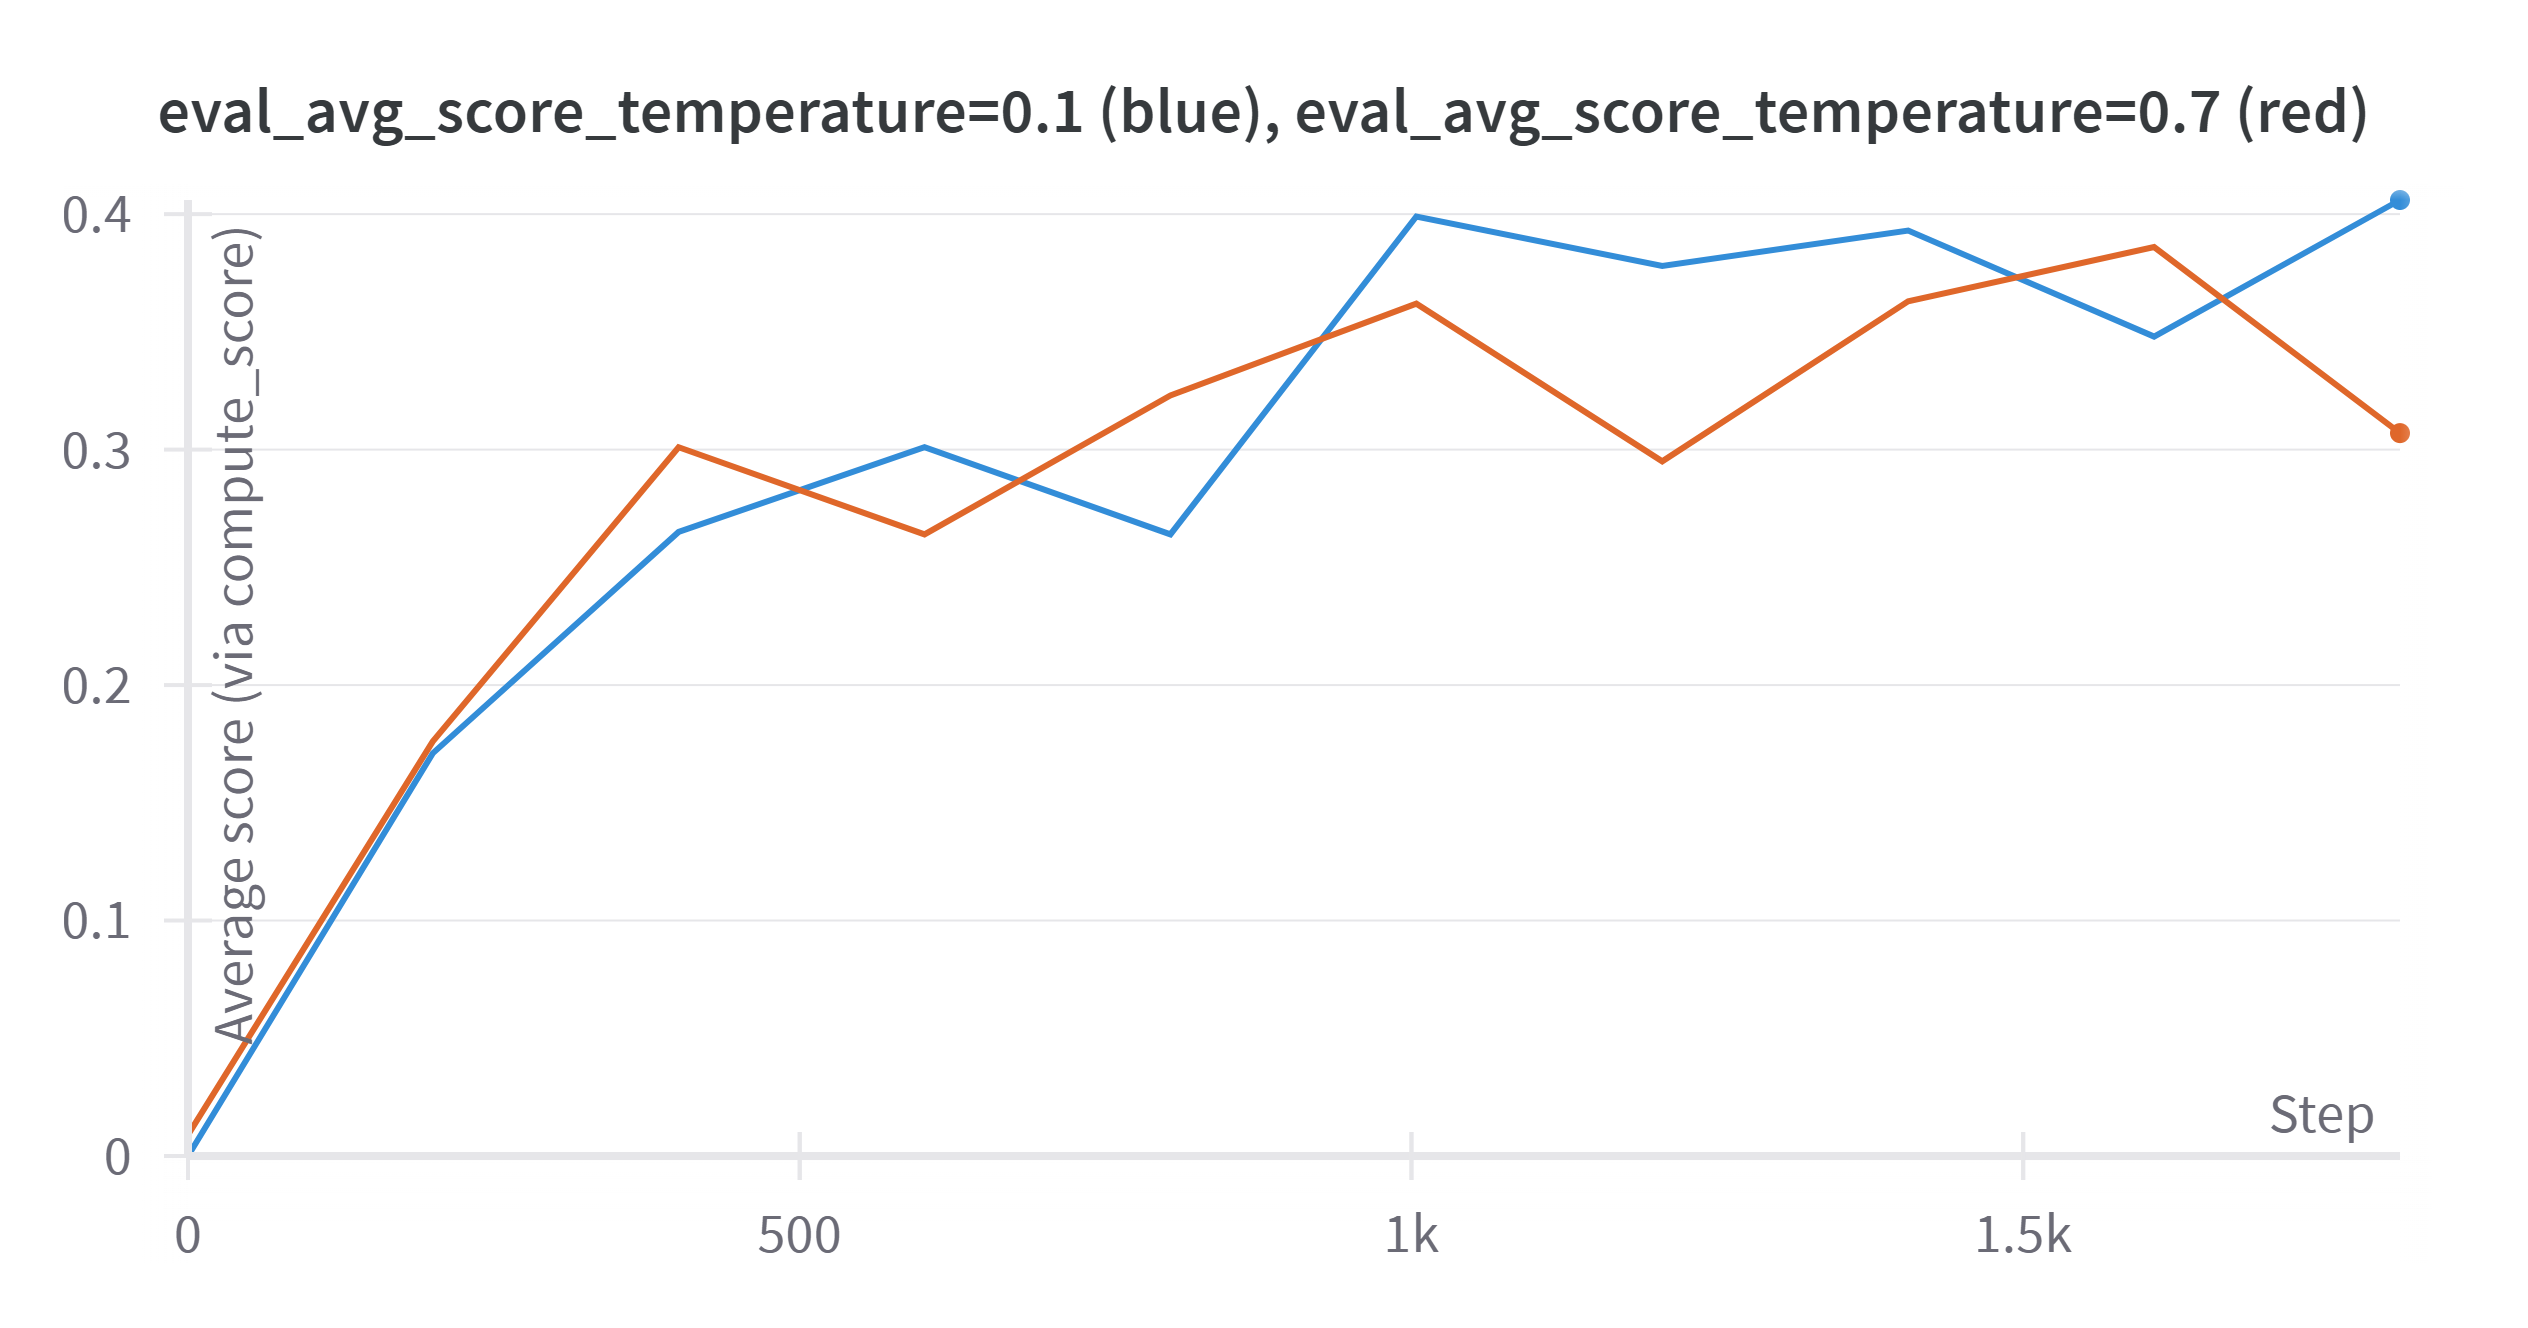
\includegraphics[width=0.8\columnwidth]{sft.png}
  \vspace{-10pt}
  \caption*{\href{https://wandb.ai/jonathanalgar/cs224r-project-sft-baseline/runs/d6osiygw/panel/w5ubogq9o}{(Click for interactive data)}}
\end{figure}

\subsubsection{Our Countdown benchmark}

We evaluate using the \texttt{compute\_score} function from ~\cite{gandhi2025cognitive} over 100 samples from a synthetic validation set\footnote{CS224R Methodological note: half the examples from the \textit{original} test set which was replaced as leaderboard evaluator before we trained this model i.e. we made an \texttt{Instruction Following} submission to the project milestone leaderboard.}. We then select the checkpoint with highest average score for \texttt{temperature=0.1} (=step 1800) as $\pi_{\theta}$ for RLOO training. For full training detail and experiment logs, see the \href{https://wandb.ai/jonathanalgar/cs224r-project-sft-baseline/runs/d6osiygw/overview}{W\&B run overview}.

\textbf{Important note}: Our SFT baseline achieves a 0.406 score on our Countdown benchmark, which is remarkably strong compared to the base model it was trained on. This means we are not operating in a truly sparse reward regime, as well over one-third of generated samples receive positive rewards even before RL fine-tuning. This strong starting point may underestimate the benefits of ATLaS compared to scenarios with genuinely sparse rewards.

\subsection{RLOO training}

For our RLOO training procedure we construct prompts (template as \texttt{\href{https://huggingface.co/datasets/Asap7772/cog_behav_all_strategies}{cog\_behav\_all\_strategies}}) from the \texttt{\href{https://huggingface.co/datasets/Jiayi-Pan/Countdown-Tasks-3to4}{Countdown-Tasks-3to4}} binary dataset (train split, \texttt{seed=42} for reproducibility). For each gradient step we sample $K=20$ candidate completions per prompt with a batch size of 8 (selected for computational feasibility). We make a fixed 101 gradient steps for the run. We use a AdamW optimizer with learning rate $\alpha = 1e^{-5}$ and KL penalty coefficient $\beta = 0$.

These are the common hyperparameters and configuration for our RLOO train runs. We want to evaluate vanilla RLOO versus RLOO+ATLAS. The configuration for the ATLaS algorithm in our experimental setup: 

\begin{itemize}
    \item Base temperature $\tau_0 = 0.7$
    \item Temperature increment $\Delta\tau = 0.1$
    \item Maximum attempts $M = 3$ ($\Rightarrow$ maximum temperature $\tau_{\max} = 0.9$)
    \item Minimum correct samples required $C_{min} = 1$
\end{itemize}

For vanilla RLOO we set $M=1$.

The headline metric will be model performance on the Countdown benchmark measured at a 20-step interval using the same protocol as outlined for our Countdown benchmark outlined above ("Best average score").

\section{Results}

The table below presents our headline experimental result as aggregated over two independent runs (1x Vanilla RLOO, 1x RLOO+ATLaS).

\begin{table}[h]
\centering
\label{tab:main_results}
\begin{tabular}{lccc}
\toprule
Method & Best average score & Relative train time \\
\midrule
Vanilla RLOO & 0.647 & 1.0x & \\
\textbf{RLOO+ATLaS} & \textbf{0.683} & 1.57x \\
\bottomrule
\end{tabular}
\end{table}

\begin{figure}[h]
  \centering
  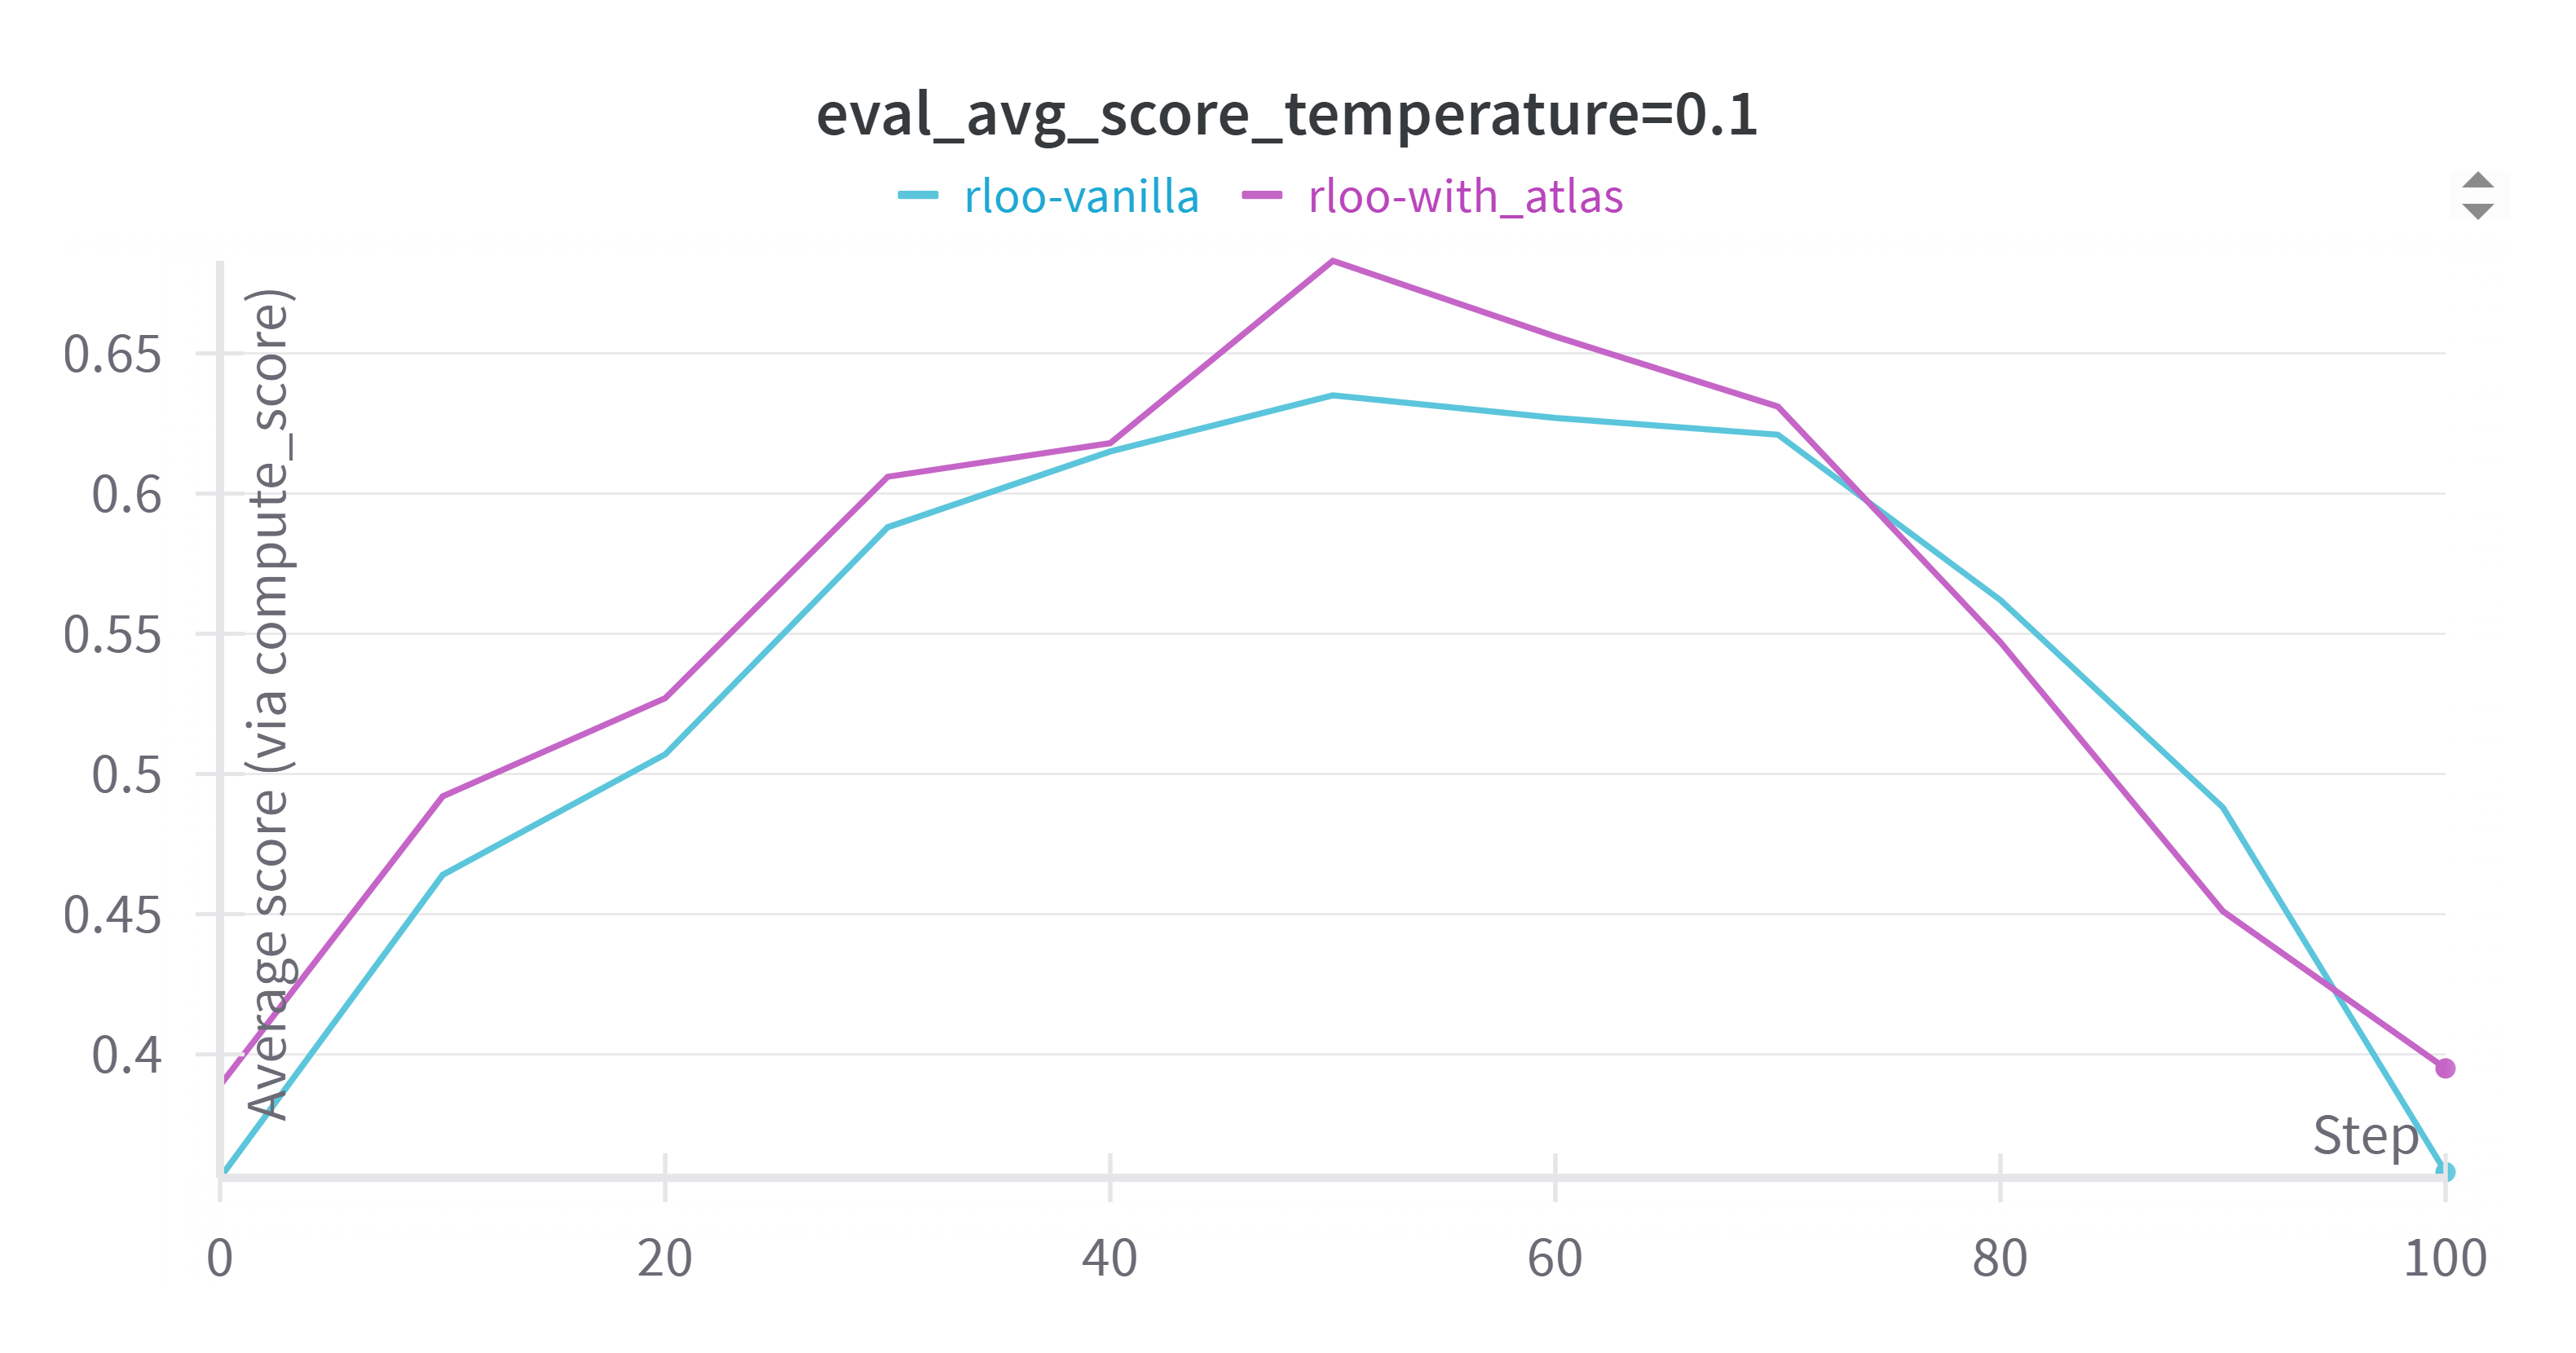
\includegraphics[width=0.8\columnwidth]{rloocomp.png}
  \vspace{-10pt}
  \caption*{\href{https://wandb.ai/jonathanalgar/countdown-rl-prod/workspace/panel/etxgwewfv}{(Click for interactive data)}}
\end{figure}

ATLaS achieves a modest \textbf{8.4\% relative improvement in best average score over vanilla RLOO.} The computational cost is significant, with a 1.57x relative increase in train time.

\textbf{Important caveat}: Due to computational budget constraints, we conducted only one training run for each method. This prevents us from establishing statistical significance or confidence intervals for the reported improvements. The observed relative improvement, while encouraging, should be interpreted as a preliminary finding requiring validation through multiple independent runs.

\subsection{Resampling}

For the \textbf{RLOO+ATLaS} run we find that of the 808 prompt (8 x 101 steps) sample sets analyzed, 306 (37.9\%) did not have correct solution after the first attempt. Of these, 35 (11.4\%) were "saved by ATLaS" and had a correct solution on the 2nd ($\tau = 0.8$, 26 prompts) or 3rd ($\tau = 0.9$, 9 prompts) attempt.

\begin{figure}[H]
  \centering
  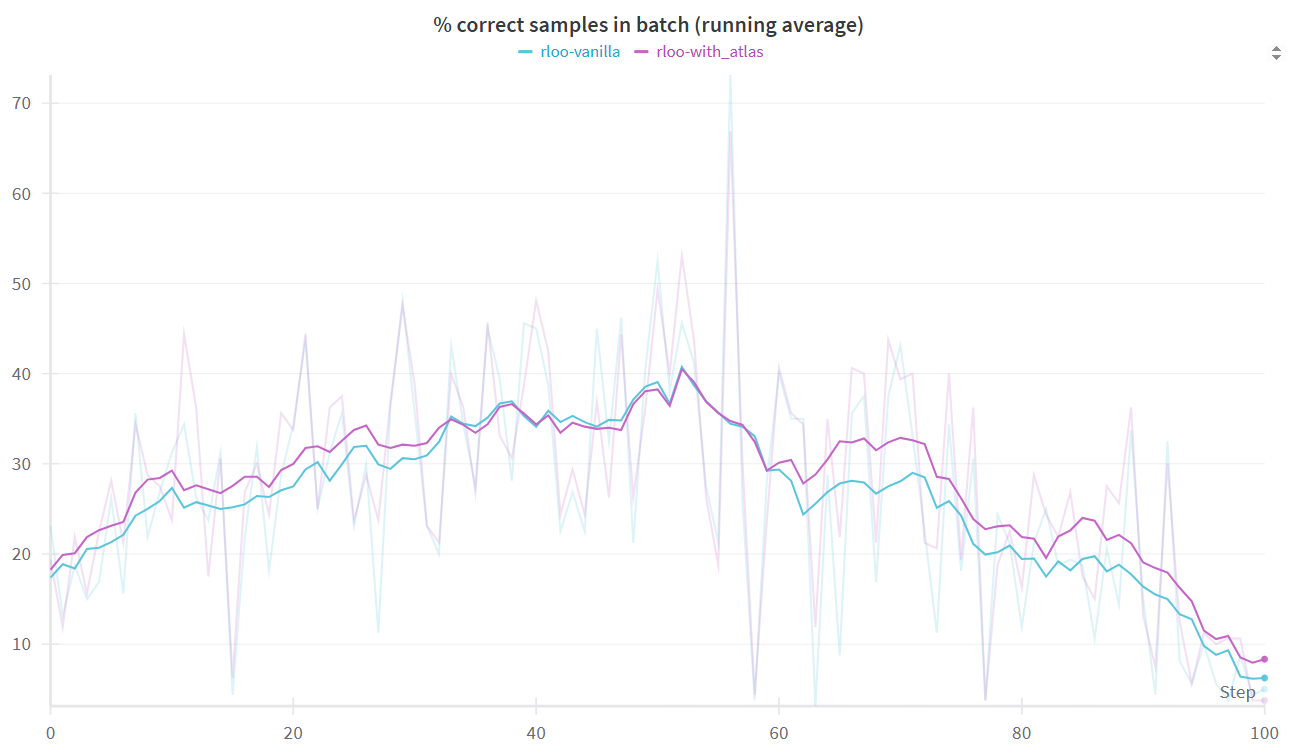
\includegraphics[width=0.8\columnwidth]{correct.png}
  \vspace{-10pt}
  \caption*{\href{https://wandb.ai/jonathanalgar/countdown-rl-prod/workspace/panel/qbxudix1v}{(Click for interactive data)}}
\end{figure}

\section{Discussion}

The temperature ladder mechanism can be understood through the lens of exploration bonuses in RL. Higher temperatures effectively implement a form of count-based exploration, encouraging the model to visit underexplored regions of the solution space. Unlike traditional exploration bonuses that require explicit state counting, temperature-based exploration emerges naturally from the sampling process.

There are several promising avenues for further research:

\textbf{Statistical validation}: The most immediate need is conducting multiple independent runs to establish statistical significance of the observed improvements and compute confidence intervals.

\textbf{Truly sparse reward settings}: Evaluating ATLaS on tasks where SFT baselines achieve near-zero performance would better demonstrate its benefits for genuinely sparse reward scenarios.

\textbf{Theoretical analysis}: Analysis of ATLaS's convergence properties and sample complexity could provide deeper insight into its effectiveness.

\section{Conclusion}

\textit{(Duplicated from extended abstract)} We introduce ATLaS, an adaptive temperature control mechanism that enhances RLOO's effectiveness on sparse-reward tasks. By systematically increasing exploration when needed, ATLaS recovers training signals from previously intractable problems, achieving an 8.4\% relative improvement on our Countdown benchmark. This work demonstrates that addressing the exploration-exploitation trade-off through adaptive sampling can improve RL fine-tuning for challenging reasoning tasks.

\paragraph{Changes from Proposal} Significant. We faced challenges with the base implementation of RLOO and its stability, so we decided to focus on an extension that does not require modifying the advantage calculation.

\bibliographystyle{ACM-Reference-Format}
\bibliography{reference}

\appendix

\section{Example train run}
\label{app:log}

Below is a snip of a train run log showing the ATLaS algorithm in action (full log \href{https://wandb.ai/jonathanalgar/countdown-rl-prod/runs/o14gnkyy/logs}{here}).\\
We see that on the first attempt only 5/8 prompts in the batch had correction solutions, but by after the third attempt 6/8 prompts have at least one correct solution. 

\begin{lstlisting}[basicstyle=\tiny\ttfamily]
...
Step 18/100

Processing batch of 8 prompt(s)
  Prompt 1: target=41 from [4, 31, 35, 62]
  Prompt 2: target=98 from [74, 28, 2, 72]
  Prompt 3: target=10 from [40, 94, 92, 5]
  Prompt 4: target=91 from [92, 91, 90]
  Prompt 5: target=39 from [66, 53, 18, 6]
  Prompt 6: target=45 from [32, 93, 16]
  Prompt 7: target=58 from [52, 7, 54, 12]
  Prompt 8: target=29 from [90, 30, 46, 15]
Using up to 3 attempts...
Generating 8 prompts x 20 samples...
After attempt 1: 37/160 correct (23.1%)
4 prompt(s) still lack correct solutions

Attempt 2/3 with temperature=0.80:
Regenerating for 4 prompts lacking correct solutions
After attempt 2: 38/160 correct (23.8%)
3 prompt(s) still lack correct solutions

Attempt 3/3 with temperature=0.90:
Regenerating for 3 prompts lacking correct solutions
After attempt 3: 39/160 correct (24.4%)

Generation phase complete...
Used 3 attempt(s), final temperature: 0.90
6/8 prompts have at least one correct solution

Sample selection summary:
  Prompt 1: Using samples from attempt 1 (temp=0.70) - 0 correct
  Prompt 2: Using samples from attempt 3 (temp=0.90) - 1 correct
  Prompt 3: Using samples from attempt 1 (temp=0.70) - 4 correct
  Prompt 4: Using samples from attempt 1 (temp=0.70) - 6 correct
  Prompt 5: Using samples from attempt 2 (temp=0.80) - 1 correct
  Prompt 6: Using samples from attempt 1 (temp=0.70) - 19 correct
  Prompt 7: Using samples from attempt 1 (temp=0.70) - 0 correct
  Prompt 8: Using samples from attempt 1 (temp=0.70) - 8 correct

Computing rewards for 8 x 20 samples...

Prompt 1 (target=41 from [4, 31, 35, 62]):
  Samples and scores:
   Sample 1: score=0.1, equation='(35 + 31) - 62'
   Sample 2: score=0.1, equation='((35 + 31) - 62) * 4'
   Sample 3: score=0.1, equation='(62 - 35) + 31'
   Sample 4: score=0.1, equation='(35 - 31) + 41'
   Sample 5: score=0.1, equation='(62 - 31) + (35 - 31)'
   Sample 6: score=0.1, equation='(31 + 35) - 62'
...
\end{lstlisting}

\end{document}